\documentclass[11pt,a4paper]{article}

%\usepackage[portuguese]{babel}  % if you want Portuguese
\usepackage[utf8]{inputenc}           % 8 bits UTF8
%\usepackage[latin1]{inputenc}     %  OR 8 bits latin1
\usepackage{parskip}            % no indentation on paragraphs
\usepackage{url}                % URLs
\usepackage[printonlyused,withpage]{acronym}
\usepackage{graphicx}
\usepackage{caption}
\usepackage{dutchcal}
\usepackage{comment}
\usepackage{amsmath} % for 'aligned' env.
\usepackage{svg} 
\usepackage{csquotes}
\usepackage{array}

\usepackage{tabularx}
\usepackage{multirow}

\newcolumntype{P}[1]{>{\centering\arraybackslash}p{#1}}


%% margins
\RequirePackage[outer=25mm,inner=30mm,vmargin=16mm,includehead,includefoot,headheight=15pt]{geometry}

%% headers and footers
\usepackage{fancyhdr}           % page headers
\pagestyle{fancy}
\lhead{}\chead{}\rhead{PD 2023/2024 Sem 1}
%\lfoot{}\cfoot{}\rfoot{Page \thepage}
\renewcommand{\headrulewidth}{0.4pt}
\renewcommand{\footrulewidth}{0.4pt}

\pagenumbering{arabic}

%% some more macros
\newcommand{\dummy}[1]{$<$#1$>$}
\newcommand{\titles}[2]{\noindent\textbf{#1:} #2\\[2mm]}

%% LaTeX exceptions
%\hyphenation{In-fra-struc-ture}

\begin{document}

\begin{comment}
    * Graph Reinforcement Learning Techniques for Improving Smart Grid Services
    * Leveraging 
\end{comment}
\titles{Title}{Graph Reinforcement Learning for Improving Smart Grid Services}
\titles{Author}{António Oliveira}
\titles{Supervision}{António Costa}
\titles{Co-Supervision}{Rosaldo Rossetti}
\titles{Date}{\today}

\section{List of Acronyms}
\begin{acronym}
    \acro{IT}{Information Technology}
    \acro{ANN}{Artificial Neural Network}
    \acro{MLP}{Multilayer Perceptron}
    \acro{CNN}{Convolutional Neural Network}
    \acro{RL}{Reinforcement Learning}
    \acro{MDP}{Markov Decision Process}
    \acro{DRL}{Deep Reinforcement Learning}
    \acro{GNN}{Graph Neural Network}
    \acro{GRL}{Graph Reinforcement Learning}
    \acro{SAC}{Soft Actor-Critic}
    \acro{DDPG}{Deep Deterministic Policy Gradient}
    \acro{DQN}{Deep Q-Network}
    \acro{PPO}{Proximal Policy Optimization}
    \acro{GCN}{Graph Convolutional Network}
    \acro{GAT}{Graph Attention Network}
    \acro{ADN}{Active Distribution Network}
\end{acronym}


\begin{comment}
    * $s, s'$ - states
    * $a$ - action
    * $r$ - reward
    * $\mathcal{S}$ - set of all nonterminal states
    * $\mathcal{S}^+$ - set of all states (including terminal state)
    * $\mathcal{A}(s)$ - set of actions available under state $s$
    * $\mathcal{R}$ - set of all possible rewards, a finite subset of \mathbb{R}
    * $\doteq$ - definition
\end{comment}

\section{Background Knowledge}

\subsection{Artificial Neural Networks}

\textbf{\acp{ANN}} are a class of machine learning algorithms based on the neural process of biological learning. The simplest form of an \ac{ANN} is a \ac{MLP}, also called a feedforward network, whose main objective is to approximate to function $f$ that models relationships between input data $x$ and output data $y$ of considerate complexity \cite{charniakIntroductionDeepLearning2018, goodfellowDeepLearning2016}. It defines a mapping $y=f(x;\theta)$ and learns the best composition of parameters $\theta$ to approximate it to the unknown model. The \ac{MLP} serves as a fundamental part of developing the other more complex types of neural networks \cite{charniakIntroductionDeepLearning2018}. \par

\subsubsection{Feedforward Neural Networks}

\begin{comment}
* Explain Loss Function
* Explain gradient descent
\end{comment}

\begin{figure}
    \centering
    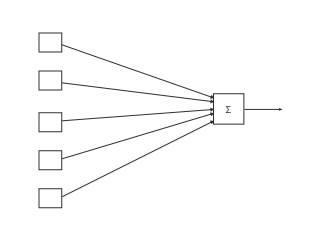
\includegraphics[width=0.50\linewidth]{PDIS/State of the Art/figures/perceptron.png}
    \caption{The Perceptron \cite{charniakIntroductionDeepLearning2018}}
    \label{fig:perceptron}
\end{figure}

The main building block of a \ac{MLP} is the \textit{Perceptron}, pictured in figure \ref{fig:perceptron}, a simple computational model initially designed as a binary classificator that mimics biological neurons' behaviour \cite{charniakIntroductionDeepLearning2018}. A neuron might have many inputs $x$ and has a single output $y$. It contains a vector of \textit{weights} $w = (w_1 ... w_m)$, each associated with a single input, and a special weight $b$ called the \textit{bias}. In this context, a perceptron defines a computational operation formulated as equation \ref{eq:perceptron} portrays \cite{charniakIntroductionDeepLearning2018}. \par

\begin{equation}\label{eq:perceptron}
f(x) =
\left\{ \begin{aligned} 
                    1 &\quad \text{ if } b + \textbf{w} \cdot \textbf{x} > 0\\
                    0 &\quad \text{ otherwise} 
                    \end{aligned} \right.
\end{equation}

Functions that compute $b + \textbf{w} \cdot \textbf{x} > 0$ are called \textit{linear units} and are identified with $\Sigma$ \cite{charniakIntroductionDeepLearning2018, goodfellowDeepLearning2016}. An activation function $g$ was introduced to enable the output of non-linear data. The default recommendation is the \textit{Rectified Linear Unit} (\textit{ReLU}), with the Logistic curve (sigmoid) also being very common \cite{goodfellowDeepLearning2016}.  \par
Feedforward networks are composed of an input layer formed by the vector of input values, an arbitrary number of hidden layers and an output layer, which is the last layer of neurons \cite{charniakIntroductionDeepLearning2018}. The greater the amount of layers the higher the \textit{depth} of the network \cite{charniakIntroductionDeepLearning2018, goodfellowDeepLearning2016}. \par
On its own, the model amounts only to a complex function. Still, with real-world correspondence between input values and associated outputs, a feedforward network can be trained to approximate the unknown function of the environment. In more concrete terms, this involves updating all of the different weight and bias values of each neuron to achieve an output as close as possible to the real or desired value or minimize the total loss, which indicates how distant the network model is to the real function to approximate \cite{charniakIntroductionDeepLearning2018, goodfellowDeepLearning2016}. \textit{Loss functions} are used to calculate this value.

\begin{figure}
    \centering
    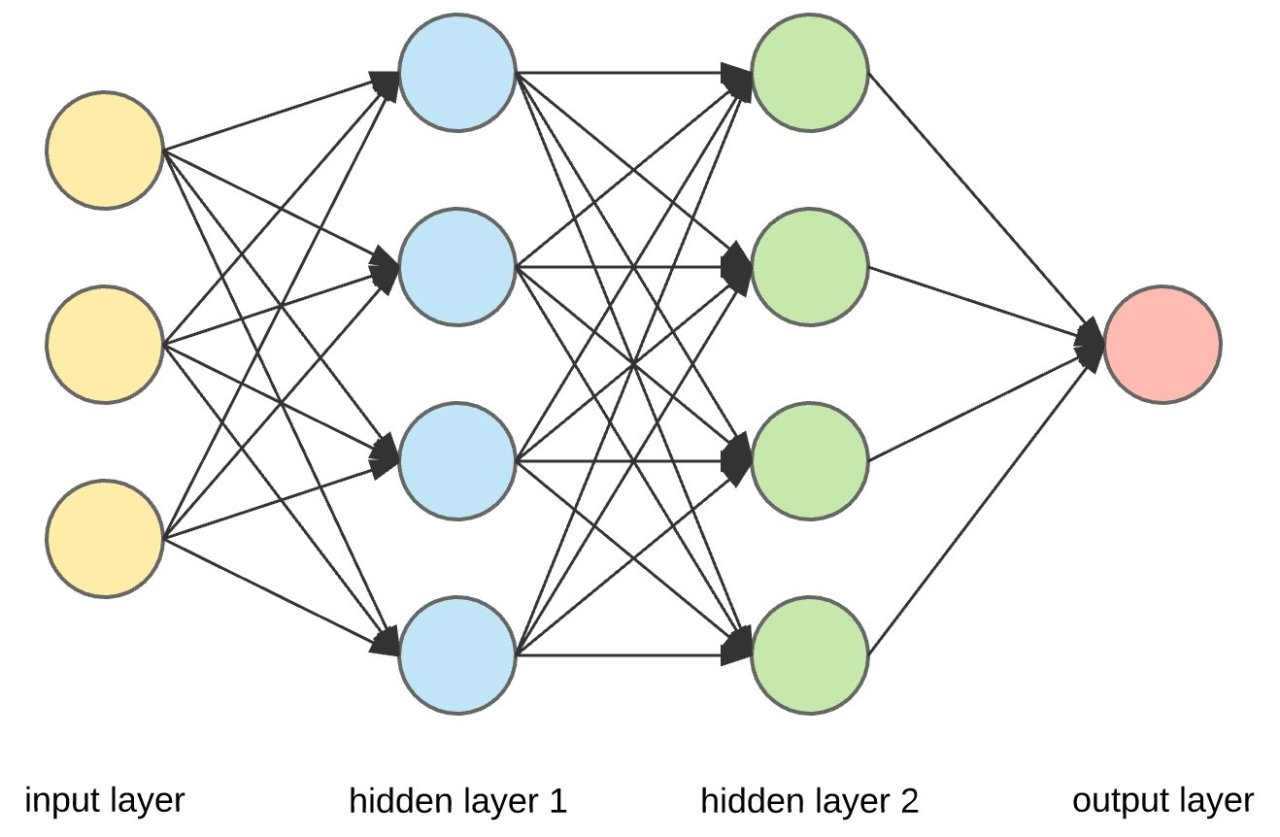
\includegraphics[width=0.50\linewidth]{PDIS/State of the Art/figures/fnn.jpg}
    \caption{Feedforward Neural Network \cite{FeedforwardNeuralNetwork}}
    \label{fig:fnn}
\end{figure}


\subsection{Reinforcement Learning}

\begin{comment}
* SAC
* DDPG
* DQN
\end{comment}

\textbf{\ac{RL}} consists of a field and a class of machine learning algorithms that study how to learn to take good sequences of actions to achieve a goal associated with a maximizing received numerical reward \cite{brunskillCS234ReinforcementLearning}. The main objective is to maximize the received cumulative reward by trying between the available actions and discovering which ones yield the most reward \cite{suttonReinforcementLearningIntroduction2014}. This sequential decision-making process becomes more complex when a delayed reward is considered, given that an action with immediate reward may not always reflect the delayed consequences of that decision \cite{suttonReinforcementLearningIntroduction2014}. It's also the learner's job to consider this during the learning process. These concepts of \textit{delayed reward} and \textit{trial-and-error search} make up the most important characteristics of Reinforcement Learning \cite{suttonReinforcementLearningIntroduction2014}. The classic formalisation of this problem is the \ac{MDP} through defining the agent-environment interaction process, explained in the following subsection \ref{section:mpd}. \par 

A major challenge in this machine learning paradigm is the trade-off between \textit{exploring} new unknown actions and \textit{exploiting} the already known "good" actions \cite{suttonReinforcementLearningIntroduction2014}. To choose the sequence of actions that return the highest reward, the agent must choose actions it found effective in similar past situations or *exploit* what it learned from experience. Furthermore, given that the agent may not know the action-reward mappings initially, it has to \textit{explore} possible actions that were not selected previously or may initially seem to yield a low reward to compute accurate reward estimates. The main problem is that neither exploitation nor exploration can be favoured exclusively without failing at the task \cite{suttonReinforcementLearningIntroduction2014}. Additionally, an agent's environment is uncertain, and changes in the environment's dynamics may also involve re-estimating action rewards. \par


In conclusion, \ac{RL} techniques enable the implementation of sequential decision-making agents that seek to maximize a reward signal analogous to an explicit (complex) goal. The agents need to balance between actions that yield a reward on posterior time steps and actions that produce immediate rewards. In addition, these agents are also faced with the task of balancing the exploitation of information from past experiences and the exploration of new decision paths that could potentially return a higher reward down the road \cite{suttonReinforcementLearningIntroduction2014}.  \par



\subsubsection{Markov Decision Process} \label{section:mpd}
\acfp{MDP} are a classical formalization of a sequential decision-making process, constituting the mathematical definition of the \ac{RL} problem \cite{suttonReinforcementLearningIntroduction2014, moralesGrokkingDeepReinforcement2020}. Beyond estimating potential rewards for the available actions, the problem defined by \acp{MDP} involves learning which actions are optimal in specific situations, i.e. learning a mapping between states of the environment and actions \cite{suttonReinforcementLearningIntroduction2014}. 

The central component of \acp{MDP} is the agent, which acts as a decision-maker and learns from interactions with the environment it's inserted. In a continuous process, the agent takes actions that affect the environment's state, which in turn presents new situations \cite{suttonReinforcementLearningIntroduction2014}. The environment also responds with the reward signals which the agent aims to maximize over time through its decision process.

\begin{figure}
    \centering
    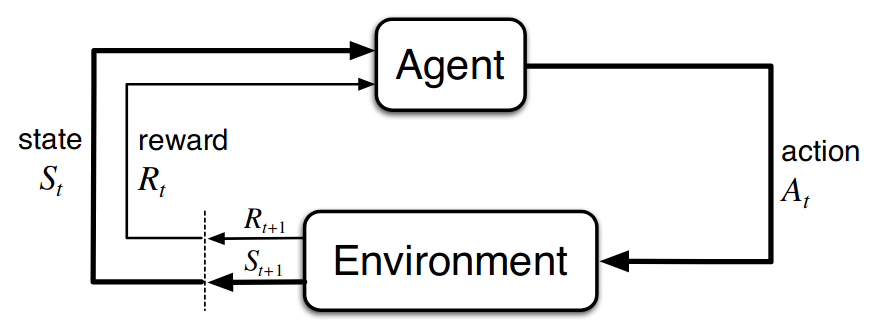
\includegraphics[width=0.75\linewidth]{PDIS/State of the Art/figures/mpd.png}
    \caption{Interaction between agent and environment in an \ac{MDP} \cite{suttonReinforcementLearningIntroduction2014}}
    \label{fig:mpd-interaction}
\end{figure}

Formally, the agent-environment interactions, as figure \ref{fig:mpd-interaction} entails, occur in a sequence of discrete time steps $t$, where at each step, the agent receives a representation of the state of the environment $S_t \in \mathcal{S}$ which is used to select an appropriate action $A_t \in \mathcal{A}(s)$, where $\mathcal{S}$ is the set of possible states called the \textit{state space} and $\mathcal{A}(s)$ is the set of available actions for state $s$ \cite{suttonReinforcementLearningIntroduction2014, moralesGrokkingDeepReinforcement2020}. In the next step, the agent receives, as a consequence of its decision, a numerical reward signal $R_{t+1} \in \mathcal{R} \subset \mathbb{R}$ and is faced with a new state $S_{t +1}$ \cite{suttonReinforcementLearningIntroduction2014}. Ultimately, the MDP agent follows a logical sequence that occurs as equation \ref{eq:mpd-sequence} states. The collection of a state $S_t$, action taken $A_{t+1}$, reward $R_{t+1}$ received and next state $S_{t+1}$ constitutes an \textit{experience tuple} \cite{moralesGrokkingDeepReinforcement2020}.

\begin{equation} \label{eq:mpd-sequence}
S_0, A_0, R_1, S_1, A_2, R_2, S_2, A_2, R_3, \dots
\end{equation}

In addition, when the set of possible actions, states and rewards ($\mathcal{A}$, $\mathcal{S}$ and $\mathcal{R}$) are finite, the \ac{MDP} is said to be \textit{finite} \cite{suttonReinforcementLearningIntroduction2014}. This results in $S_t$ and $R_t$ having well-defined discrete probability distributions in function of the preceding state and chosen action \cite{suttonReinforcementLearningIntroduction2014}. Therefore, the probability of receiving a particular reward and state given the previous state and selected action, which characterizes a finite MPD's dynamics, may be characterized by function $p$ defined in equation \ref{eq:mdp-dynamics}
\begin{equation} \label{eq:mdp-dynamics}
p(s',r|s,a) \doteq Pr\{S_t = s', R_t = r | S_{t-1} = s, A_{t-1} = a\}
\end{equation}

For all $s, s' \in \mathcal{S}$, $r \in \mathcal{R}$ and $a \in \mathcal{A}(s)$, where $\doteq$ denotes a mathematical formal defintion. This encompasses the assumption that the probability of each possible state, $S_t$, and reward, $R_t$, pair is only dependent on the preceding state, $S_{t-1}$, and action taken, $A_{t-1}$ \cite{suttonReinforcementLearningIntroduction2014}. Instead of observing this as a restriction on the decision process, it's more convenient to view it as a constraint on the state variable, considering that it must contain all the necessary information from experience to make a valuable decision in the immediate step. If this condition is satisfied, the state is declared to have the \textit{markov property} \cite{suttonReinforcementLearningIntroduction2014}. \par
From function $p$ in equation \ref{eq:mdp-dynamics}, the state-transtion probabilities, also called the \textit{transition function}, can be computed as described by equation \ref{eq:mpd-transition} \cite{suttonReinforcementLearningIntroduction2014, moralesGrokkingDeepReinforcement2020}.

\begin{equation} \label{eq:mpd-transition}
    p(s'|s,a) \doteq Pr\{S_t = s'|S_{t-1} = s, A_{t-1} = a\} = \sum_{r \in \mathcal{R}} p(s',r|s,a)
\end{equation}

In addition, the expected rewards can be calculated for state-action pairs (equation \ref{eq:mpd-reward-sa}) or state-action-next-action triples (equation \ref{eq:mpd-reward-sas'}) \cite{suttonReinforcementLearningIntroduction2014, moralesGrokkingDeepReinforcement2020}.

\begin{equation} \label{eq:mpd-reward-sa}
    r(s,a) \doteq \mathbb{E}[R_t | S_{t-1} = s, A_{t-1} = a] = \sum_{r \in \mathcal{R}} r \sum_{s' \in \mathcal{S}} p(s', r|s,a)
\end{equation}
\begin{equation} \label{eq:mpd-reward-sas'}
    r(s,a,s') \doteq \mathbb{E}[R_t | S_{t-1} = s, A_{t-1} = a, S_t = s'] = \sum_{r \in \mathcal{R}} r \frac{p(s',r|s,a)}{p(s'|s,a)}
\end{equation}

\subsubsection{Rewards and Returns}

As stated in the previous subsections, the main goal of a \ac{RL} agent defined by the numeric reward signal, $R_t \in \mathbb{R}$, it receives from the environment \cite{suttonReinforcementLearningIntroduction2014}. In this context, the agent's objective is to maximize the total reward it receives, considering not only immediate but also the cumulative reward over time. In the ubiquitous work of \cite{suttonReinforcementLearningIntroduction2014}, the \textit{reward hypothesis} is stated as follows:

\begin{displayquote}
That all of what we mean by goals and purposes can be well thought of as the maximization of the expected value of the cumulative sum of a received scalar signal (called reward). \cite{suttonReinforcementLearningIntroduction2014}
\end{displayquote}
This also entails that the process of reward maximization from the agent has to be closely tied to it achieving its defined goals in a practical sense. Otherwise, the agent will fail at fulfilling the desired objectives \cite{suttonReinforcementLearningIntroduction2014}.

Formally, the goal of an \ac{RL} agent can be defined by the maximization of the cumulative reward received of time called the \textit{expected return}, $G_t$ \cite{suttonReinforcementLearningIntroduction2014}.

\begin{equation} \label{eq:expected-return}
    G_t \doteq R_{t+1} + R_{t+2} + R_{t+3} + \cdots + R_T
\end{equation}

$T$ describes the final time step. This definition can be applied in domains with a natural notion of a terminal state or final time step. In these cases, the agent-environment interaction process can be broken into logically independent subsequences called \textit{episodes} \cite{suttonReinforcementLearningIntroduction2014}. Each episode ends in a special state, called the terminal state, restarting a new sequence of states and actions completely independent from the previous episode \cite{suttonReinforcementLearningIntroduction2014}. In this context, episodes can be considered to end in the same terminal state, with different accumulated rewards for the different outcomes \cite{suttonReinforcementLearningIntroduction2014}.

In contrast, there are situations where the decision-making process doesn't divide itself into logically identifiable episodes but goes on indefinitely. In this case, $T = \infty$ and according to equation \ref{eq:expected-return}, the expected return the agent aims to maximize would be infinite \cite{suttonReinforcementLearningIntroduction2014}. In this manner, another concept is added in the expected return definition called the \textit{discount rate}, $\gamma$ where $0 \leq \gamma \leq 1$, representing how strongly the agent should account for future rewards in the expected return calculations, as equation \ref{eq:expected-discounted-return} \cite{suttonReinforcementLearningIntroduction2014}.

\begin{equation} \label{eq:expected-discounted-return}
    G_t \doteq R_{t+1} + \gamma R_{t+2} + \gamma^2 R_{t+3} + \cdots = \sum^\infty_{k = 0} \gamma^k R_{t+k+1}
\end{equation}

From this equation, we can compute the expected discounted return on a given time step $t$ in the function of the immediate reward signal received and the expected return for the next time step $t +1$, which eases the job of calculating expected returns for reward sequences \cite{suttonReinforcementLearningIntroduction2014}. This is entailed by equation \ref{eq:expected-discounted-next}.
\begin{equation} \label{eq:expected-discounted-next}
    G_t = R_{t+1} + \gamma G_{t+1}
\end{equation}

In this manner, a \ac{MDP} can be defined by a tuple with a state space $\mathcal{S}$, an action space $\mathcal{A}$, a transition function $p$, a reward function $r$ and a discount factor $\gamma$, as equation \ref{eq:mdp-tuple} portrays \cite{brunskillCS234ReinforcementLearning}.

\begin{equation} \label{eq:mdp-tuple}
    M = (\mathcal{S}, \mathcal{A}, p, r, \gamma)
\end{equation}

\subsubsection{Policies and Value Functions}

\ac{RL} techniques typically involve the estimation of what is understood as \textit{value functions}, functions that estimate the expected return based on the current state value or state-action pair. This characterizes how good is for an agent to be in a specific state or to take an action in a specific state, respectively, using the expected return to characterize the overall \textit{goodness} of these scenarios \cite{suttonReinforcementLearningIntroduction2014, moralesGrokkingDeepReinforcement2020}. These functions are tied to a specific way of determining the action in a given state. Formally, this is defined as a \textit{policy} $\pi$, that defines the probability $\pi(a|s)$ of taking action $a$ in state $s$ \cite{suttonReinforcementLearningIntroduction2014}. In this context, the \textit{state-value function}, $v_\pi(s)$ and \textit{action-value functions} $q_\pi(s,a)$ for policy $\pi$ can be defined by equations \ref{eq:state-value-funtion} and \ref{eq:action-value-function}, respectively \cite{suttonReinforcementLearningIntroduction2014}.
\begin{equation} \label{eq:state-value-funtion}
    v_\pi(s) \doteq \mathbb{E}_\pi[G_t | S_t = s], \forall s \in \mathcal{S}
\end{equation}
\begin{equation} \label{eq:action-value-function}
    q_\pi(s,a) \doteq \mathb{E}_\pi[G_t | S_t = s, A_t = a]    
\end{equation}

The utility of such functions rely on the possibility of estimating them with regard to past experience of the agent \cite{suttonReinforcementLearningIntroduction2014}. A fundamental property of value functions is that it can, as was the case with the expected return (equation \ref{eq:expected-discounted-next}), satisfy recursive relationships with the next immediate value as equation \ref{eq:bellman-equation-v} entails \cite{suttonReinforcementLearningIntroduction2014}. This equation is called the \textit{Bellman equation for $v_\pi$}, which characterizes the relationship between the value of current and subsequent states.

\begin{equation} \label{eq:bellman-equation-v}
    v_\pi \doteq \sum_{a \in \mathcal{A}(s)} \pi(a|s) \sum_{s' \in \mathcal{S}, r \in \mathcal{R}} p(s',r|s,a) [r + \gamma v_\pi (s')]
\end{equation}
\begin{equation} \label{eq:action-value-function}
    q_\pi(s,a) \doteq \sum\mathbb{E}_\pi[G_t | S_t = s, A_t = a]    
\end{equation}


\subsubsection{Types of \ac{RL}}


\begin{figure}
    \centering
    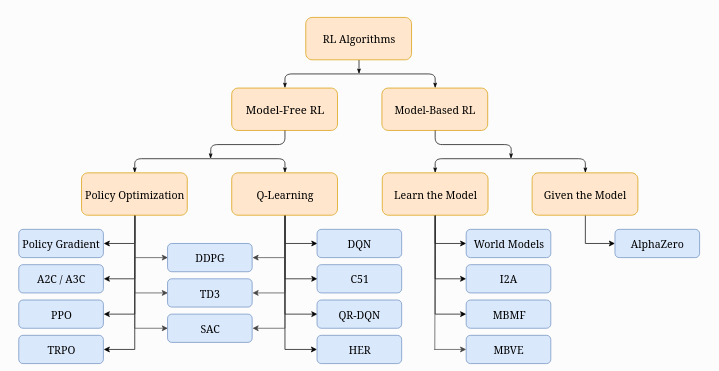
\includegraphics[width=0.75\linewidth]{PDIS/State of the Art/figures/rl_algorithms.png}
    \caption{Taxonomy of algorithms in modern \ac{RL} \cite{openaiSpinningDocumentation}}
    \label{fig:rl-algorithms}
\end{figure}

Regarding \ac{RL} algorithms, they can be divided into model-free and model-based techniques \cite{openaiSpinningDocumentation}. These categories are distinguished by whether an agent uses a provided or learned \textit{model} of the set of transition and reward functions, another optional element of \ac{RL} techniques \cite{moralesGrokkingDeepReinforcement2020, openaiSpinningDocumentation}. In the positive case, the method is said to be model-based, otherwise, it's model-free. Having an accurate model of the environment allows the \ac{RL} agent to focus on planning ahead by calculating future scenarios and creating policies based on the results of the planning process. An example of a famous system of this kind is AlphaZero \cite{silverMasteringChessShogi2017}. However, in most cases, agents can't access a ground-truth model of the environment, leaving only the scenario where an agent learns a model purely from experience. This creates several challenges, the most prominent of which relies on the fact that the model, in most times, doesn't fully capture the environment's transition dynamics, equipping it with bias in relation to the actual dynamics. With this, learning how to generalise the model to real-world environments so that the bias is not over-exploited becomes a very complex task \cite{openaiSpinningDocumentation}.  Model-free algorithms can be also further divided into Q-learning and Policy Aproximmation techniques. \par
Furthermore, algorithms can also be subdivided into on-policy and off-policy methods. \cite{moralesGrokkingDeepReinforcement2020} On-policy algorithms evaluate and improve a single policy used to determine the agent's behaviour \cite{moralesGrokkingDeepReinforcement2020}. The methods under the policy optimization category such as A2C and A3C \cite{mnihAsynchronousMethodsDeep2016} or the \ac{PPO} \cite{schulmanProximalPolicyOptimization2017} almost always fall into this label. In contrast, off-policy algorithms learn how to improve a different target policy based on the results that arise from the policy used to determine the system behaviour initially \cite{moralesGrokkingDeepReinforcement2020}. Such approaches include Q-Learning algorithms such as \acp{DQN} \cite{mnihHumanlevelControlDeep2015, openaiSpinningDocumentation}. \ac{DDPG} \cite{lillicrapContinuousControlDeep2019} combines policy optimization with q-learning, consisting of an off-policy method that learns both a q-function and a policy. \ac{DDPG} constitutes the adaption of q-learning methods to continuous action spaces \cite{openaiSpinningDocumentation}. Another example of an off-policy algorithm is the \ac{SAC} \cite{haarnojaSoftActorCriticOffPolicy2018} method, which bridges stochastic policy optimization with the \ac{DDPG} approach and has entropy regularization as one of its central features, which translates into training a policy that maximizes the expected return and entropy, a measure of randomness in the policy \cite{openaiSpinningDocumentation}. \par
Lastly, with the advent of deep learning becoming one of the most ubiquitous techniques in machine learning, \ac{RL} algorithms have evolved beyond the traditional tabular methods \cite{moralesGrokkingDeepReinforcement2020}. Traditional \ac{RL} has evolved to \ac{DRL}, which studies how to use deep neural networks in \ac{RL} problems to leverage their generalization abilities for solving more complex problems.

\subsection{Graph Representation Learning}

Several objects and problems can be naturally expressed in the real world using graphs, such as social networks, power grids, transportation networks, recommendation systems or drug discovery. The usefulness of such representations is tied to how they instinctively represent the complex relationships between objects. However, graph data is often very sparse and complex, and their sophisticated structure is difficult to deal with \cite{liuIntroductionGraphNeural2020, zhaoRepresentationLearning2022}. \par

Furthermore, the performance of machine learning models strongly relies not only on their design but also on good representations of the underlying information \cite{liuIntroductionGraphNeural2020}.  Ineffective representations, on the one hand, can lack important graph features and, on the other, can carry vast amounts of redundant information, affecting the algorithms' performance in leveraging the data for different analytical tasks \cite{liuIntroductionGraphNeural2020, wuGraphNeuralNetworks2022}. \par

In this context, \textbf{Graph Representation Learning} studies how to learn the underlying features of graphs to extract a minimal but sufficient representation of the graph attributes and structure \cite{hamiltonGraphRepresentationLearning, zhaoRepresentationLearning2022, cuiGraphRepresentationLearning2022}. Currently, the improvements in deep learning allow representation learning techniques consisting of the composition of multiple non-linear transformations that yield more abstract and, ultimately, more useful representations of graph data \cite{cuiGraphRepresentationLearning2022}. 

\subsection{Graph Neural Networks}

\begin{comment}
* GraphSAGE
\cite{scarselliGraphNeuralNetwork2009}
\end{comment}

In the present, deep learning and \ac{ANN} have become one of the most prominent approaches in Artificial Intelligence research \cite{cuiGraphRepresentationLearning2022}. Approaches such as recurrent neural networks and convolutional networks have achieved remarkable results on Euclidean data, such as images or sequence data, such as text and signals \cite{wuGraphNeuralNetworks2022a}. Furthermore, techniques regarding deep learning applied to graphs have also experienced rising popularity among the research community, more specifically \textbf{\acp{GNN}} that became the most successful learning models for graph-related tasks across many application domains \cite{cuiGraphRepresentationLearning2022, wuGraphNeuralNetworks2022a}. \par

The main objective of \acp{GNN} is to update node representations with representations from their neighbourhood iteratively \cite{tangGraphNeuralNetworks2022}. Starting at the first representation $H^0 = X$, each layer encompasses two important functions:
\begin{itemize}
    \item \textbf{Aggregate}, in each node, the information from their neighbours
    \item \textbf{Combine} the aggregated information with the current node representations
\end{itemize}

The general framework of \acp{GNN}, outlined in \cite{tangGraphNeuralNetworks2022}, can be defined mathematically as follows: \\ \\
Initialization: $H^0 = X$ \\
For $k = 1, 2, \dots, K$
\begin{gather*}
 a^k_v = \text{AGGREGATE}^k\{H^{k-1}_u : u \in N(v)\} \\
 H^k_v = \text{COMBINE}^k\{H^{k-1}_u, a^k_v\}       
\end{gather*}

Where $N(v)$ is the set of neighbours for the $v$-th node. The node representations $H^K$ in the last layer can be treated as the final representations, which sequentially can be used for other downstream tasks \cite{tangGraphNeuralNetworks2022}.


\subsubsection{Graph Convolutional Network}

A \textbf{\ac{GCN}} \cite{kipfSemiSupervisedClassificationGraph2017} is a popular architecture of \acp{GNN} praised by its simplicity and effectiveness in a variety of tasks \cite{liuIntroductionGraphNeural2020, tangGraphNeuralNetworks2022}. In this model, the node representations in each layer are updated according to the following convolutional operation:

\begin{equation} \label{eq:graph-convolution}
  H^{k+1} = \sigma(\tilde{D}^{-\frac{1}{2}} \tilde{A} \tilde{D}^{-\frac{1}{2}} H^k W^k)  
\end{equation}

$Ã = A + I$ - Adjacency Matrix with self-connections \\
$I \in \mathbb{R}^{N \times N}$ - Identity Matrix \\
$\tilde{D}$ - Diagonal Matrix,  with $\tilde{D}_{ii} = \sum_j Ã_{ij}$ \\
$\sigma$ - Activation Function \\
$W^k \in \mathbb{R}^{F \times F'}$ - Laywise linear transformation matrix ($F$ and $F'$ are the dimensions of node representations in the $k$-th and $(k + 1)$ layer, respectively) \\
 
$W^k \in \mathbb{R}^{F \times F'}$ is a layerwise linear transformation matrix that is trained during optimization \cite{tangGraphNeuralNetworks2022}. The previous equation \ref{eq:graph-convolution} can be dissected further to understand the \textit{AGGREGATE} and \textit{COMBINE} function definitions in a \ac{GCN} \cite{tangGraphNeuralNetworks2022}. For a node $i$, the representation updating equation can be reformulated as:

\begin{gather}
    H^k_i = \sigma(\sum_{j \in \{N(i) \cup i\}} \frac{\tilde{A}_{ij}}{\sqrt{\tilde{D}_{ii} \tilde{D}_{jj}}} H^{k-1}_j W^k) \\
    H^k_i = \sigma(\sum_{j \in N(i)} \frac{A_{ij}}{\sqrt{\tilde{D}_{ii} \tilde{D}_{jj}}} H^{k-1}_j W^k) + \frac{1}{\tilde{D}_i} H^{k-1} W^k)
\end{gather}

In the second equation, the \textit{AGGREGATE} function can be observed as the weighted average of the neighbour node representations \cite{tangGraphNeuralNetworks2022}. The weight of neighbour $j$ is defined by the weight of the edge $(i,j)$, more concretely, $A_{ij}$ normalized by the degrees of the two nodes \cite{tangGraphNeuralNetworks2022}. The \textit{COMBINE} function consists of the summation of the aggregated information and the node representation itself, where the representation is normalized by its own degree \cite{tangGraphNeuralNetworks2022}.

\subsubsection*{Spectral Graph Convolutions}

Regarding the connection between GCNs an spectral filters defined on graphs, spectral convolutions can be defined as the multiplication of a node-wise signal $x \in \mathbb{R}^N$ with a convolutional filter $g_\theta = diag(\theta)$ in the \textit{Fourier domain} \cite{liuIntroductionGraphNeural2020, tangGraphNeuralNetworks2022}, formally:

\begin{equation}    
g_\theta \star \text{x} = U_{g_\theta} U^T \text{x}
\end{equation}

$\theta \in \mathbb{R}^N$ - Filter parameter \\
$U$ - Matrix of eigenvectors of the normalized graph Laplacian Matrix $L = I_N - D^{-\frac{1}{2}} AD^{-\frac{1}{2}}$ \\

 The eigendecomposition of the Laplacian matrix can also be defined by $L = U \Lambda U^T$ with $\Lambda$ serving as the diagonal matrix of eigenvalues and $U^T \text{x}$ is the graph Fourier transform of the input signal $\text{x}$ \cite{tangGraphNeuralNetworks2022}. In a practical context, $g_\theta$ is the function of eigenvalues of the normalized graph Laplacian matrix $L$, that is $g^\theta(\Lambda)$ \cite{liuIntroductionGraphNeural2020, tangGraphNeuralNetworks2022}. Computing this is a problem of quadratic complexity to the number of nodes $N$, something that can be circumvented by approximating $g_\theta (\Lambda)$ with a truncated expansion of Chebyshev polynomials $T_k(x)$ up to $K$-th order \cite{liuIntroductionGraphNeural2020, tangGraphNeuralNetworks2022}:

\begin{equation}
g_{\theta'}(\Lambda) = \sum^K_{k=0} \theta'_k T_k(\tilde{\Lambda})    
\end{equation}
 
$\tilde{\Lambda} = \frac{2}{\lambda_\text{max}} \Lambda - \text{I}$  \\
$\lambda_\text{max}$ - Largest eigenvalue of $L$ \\
$\theta' \in \mathbb{R}^N$ - Vector of Chebyshev coefficients \\
$T_k(x)$ - Chebyshev polynomials \\
$T_k(x) = 2 x T_{k - 1} (x) - T_{k - 2}(x)$ with $T_0(x) = 1$ and $T_1(x) = x$ \\

By combining this with the previous equation, the first can be reformulated as:

\begin{equation}
g_\theta \star \text{x} = \sum^K_{k=0} \theta'_k T_k(\tilde{L}) \text{x}
\end{equation}
 
 $\tilde{L} = \frac{2}{\lambda_\text{max}} L - I$ 

From this equation, it can be observed that each node depends only on the information inside the $K$-th order neighbourhood and with this reformulation, the computation of the equation is reduced to $O(|\xi|)$, linear to the number of edges $\xi$ in the original graph $G$. \par

To build a neural network with graph convolutions, it's sufficient to stack multiple layers defined according to the previous equation, each followed by a nonlinear transformation. However, the authors of \ac{GCN} \cite{kipfSemiSupervisedClassificationGraph2017} proposed limiting the convolution number to $K = 1$ at each layer instead of limiting it to the explicit parametrization by the Chebyshev polynomials. This way, each level only defines a linear function over the Laplacian Matrix $L$, maintaining the possibility of handling complex convolution filter functions on graphs by stacking multiple layers \cite{kipfSemiSupervisedClassificationGraph2017, tangGraphNeuralNetworks2022}. This means the model can alleviate the overfitting of local neighbourhood structures for graphs whose node degree distribution has a high variance \cite{kipfSemiSupervisedClassificationGraph2017, tangGraphNeuralNetworks2022}.

At each layer, it can further considered $\lambda_\text{max} \approx 2$, which the neural network parameters could accommodate during training \cite{tangGraphNeuralNetworks2022}. With these simplifications, the equation is transformed into:
\begin{equation}
g_{\theta'} \star \text{x} \approx \theta'_0 \text{x} + \theta'_1 \text{x} (L - I_N) \text{x} = \theta'_0 \text{x} - \theta'_1 D^{-\frac{1}{2}} AD^{-\frac{1}{2}}
\end{equation}
 
 $\theta'_0$ and $\theta'_1$ - Free parameters that can be shared over the entire graph \\


The number of parameters can, in practice, be further reduced, minimising overfitting and minimising the number of operations per layer as well \cite{tangGraphNeuralNetworks2022} as equation \ref{eq:gcn-reduced-param} entails.

\begin{equation} \label{eq:gcn-reduced-param}
g_\theta \star \text{x} \approx \theta (I + D^{-\frac{1}{2}} AD^{-\frac{1}{2}}) \text{x}
\end{equation}
 
$\theta = \theta'_0 = - \theta'_1$

One potential problem is the $I_N + D^{-\frac{1}{2}} AD^{-\frac{1}{2}}$ matrix whose eigenvalues fall in the $[0,2]$ interval. In a deep GCN, the repeated utilization of the above function often leads to an exploding or vanishing gradient, translating into numerical instabilities \cite{liuIntroductionGraphNeural2020, tangGraphNeuralNetworks2022}. In this context, the matrix can be further renormalized by converting $I + D^{-\frac{1}{2}} AD^{-\frac{1}{2}}$ into $\tilde{D}^{-\frac{1}{2}} \tilde{A}\tilde{D}^{-\frac{1}{2}}$ \cite{liuIntroductionGraphNeural2020, tangGraphNeuralNetworks2022}. 
In this case, only the scenario where there is one feature channel and one filter is considered which can be then generalized to an input signal with $C$ channels $X \in \mathbb{R}^{N \times C}$ and $F$ filters (or hidden units) \cite{liuIntroductionGraphNeural2020, tangGraphNeuralNetworks2022}:
\begin{equation}
H = \tilde{D}^{-\frac{1}{2}} \tilde{A}\tilde{D}^{-\frac{1}{2}}XW    
\end{equation}

$W \in \mathbb{R}^{C \times F}$ - Matrix of filter parameters \\
$H$ - Convolved Signal Matrix \\


\subsubsection{Graph Attention Network}

\textbf{\ac{GAT}} \cite{velickovicGraphAttentionNetworks2018} is another type of \acp{GNN} that focuses on leveraging an attention mechanism to learn the importance of a node's neighbours. In contrast, the \ac{GCN} uses edge weight as importance, which may not always represent the true strength between two nodes \cite{tangGraphNeuralNetworks2022, velickovicGraphAttentionNetworks2018}.

The Graph Attention Layer defines the process of transferring the hidden node representations at layer $k - 1$ to the next node presentations at $k$. To ensure that sufficient expressive power is attained to allow the transformation of the lower-level node representations to higher-level ones, a linear transformation $W \in \mathbb{R}^{F \times F'}$ is applied to every node, followed by the self-attention mechanism, which measures the attention coefficients for any pair of nodes through a shared attentional mechanism $a: \mathbb{R}^{F'} \times \mathbb{R}^{F'} \rightarrow \mathbb{R}$ \cite{tangGraphNeuralNetworks2022, velickovicGraphAttentionNetworks2018}. In this context, relationship strength $e_{ij}$ between two nodes $i$ and $j$ can be calculated by:
\begin{equation}
e_{ij} = a(W H^{k - 1}_i, W H^{k - 1}_j)
\end{equation}

$H^{k - 1}_i \in \mathbb{R}^{N \times F'}$ - Column-wise vector representation of node $i$ at layer $k - 1$ ($N$ is the number of nodes and $F$ the number of features per node) \\
$W \in \mathbb{R}^{F \times F'}$ - Shared linear transformation \\
$a: \mathbb{R}^{F'} \times \mathbb{R}^{F'} \rightarrow \mathbb{R}$ - Attentional Mechanism \\
$e_{ij}$ - Relationship Strength between nodes $i$ and $j$ \\

Theoretically, each node can attend to every other node on the graph, although it would ignore the graph's topological information in the process. A more reasonable solution is to only attend nodes in the neighbourhood \cite{velickovicGraphAttentionNetworks2018, tangGraphNeuralNetworks2022}. In practice, only first-order node neighbours are used, including the node itself, and to make the attention coefficients comparable across the various nodes, they are normalized with a \textit{softmax} function:
$$ \alpha_{ij} = \text{softmax}_j(\{e_{ij}\}) = \frac{exp(e_{ij})}{\sum_{l \in N(i)} exp(e_{il})}$$
 
Fundamentally, $\alpha_{ij}$ defines a multinomial distribution over the neighbours of node $i$, which can also be interpreted as a transition probability from node $i$ to each node in its neighbourhood \cite{tangGraphNeuralNetworks2022}. 
In the original work \cite{velickovicGraphAttentionNetworks2018}, the attention mechanism is defined as a single-layer Feedforward Neural Network that includes a linear transformation with weigh vector $W_2 \in \mathbb{R}^{1 \times 2 F'}$ and a LeakyReLU nonlinear activation function with a negative input slope $\alpha = 0.2$ \cite{tangGraphNeuralNetworks2022, velickovicGraphAttentionNetworks2018}. More formally, the attention coefficients are calculated as follows:
\begin{equation}
    \alpha_{ij} = \frac{ \text{exp}( \text{LeakyReLU}( W_2 [W H^{k - 1}_i || W H^{k - 1}_j]))}{ \sum_{l \in N(i)} \text{exp}( \text{LeakyReLU}( W_2 [W H^{k - 1}_i || W H^{k - 1}_l])) }
\end{equation}
 
$||$ - Vector concatenation operation

The novel node representation is a linear composition of the neighbouring representations with weights determined by the attention coefficients \cite{velickovicGraphAttentionNetworks2018, tangGraphNeuralNetworks2022}, formally:
\begin{equation}
    H^k_i = \sigma(\sum_{j \in N(i)} \alpha_{ij} W H^{k - 1}_j) 
\end{equation}
 

\subsubsection*{Multi-head Attention}

Multi-head attention can be used instead of self-attention, determining a different similarity function over the nodes. An independent node representation can be obtained for each attention head according to the equation bellow \cite{velickovicGraphAttentionNetworks2018, tangGraphNeuralNetworks2022}. The final representation is a concatenation of the node representations learned by different heads, formally:
$$ H^k_i = \Big\Vert^T_{t=1} \sigma(\sum_{j \in N(i)} \alpha^t_{ij} W^t H^{k-1}_j)$$
 
$T$ - Number of attention heads \\
$\alpha^t_{ij}$ - attention coefficient computed from the $t$-th attention head \\
$W^t$ - Linear transformation matrix of the $t$-th attention head \\

Lastly, the author also mentions that other pooling techniques can be used in the final layer for combining the node representations from different heads, for example, the average node representations from different attention heads \cite{velickovicGraphAttentionNetworks2018, tangGraphNeuralNetworks2022}.
\begin{equation}
    H^k_i = \sigma(\frac{1}{T} \sum^T_{t = 1} \sum_{j \in N(i)} \alpha^t_{ij} W^t H^{k-1}_j)
\end{equation}
 

\subsection{Smart Grid Services}

Given the global ecological emergency and the increasing energetic crisis, there is a necessity for advancements in energy distribution and transmission systems now more than ever. To fulfil the need for energy sustainability, traditional centralized distribution grids must be adapted to, on the one hand, accommodate the rise of distributed renewable energy sources in corporate and domestic consumers and, on the other, to make more efficient and reliable distribution of energy resources \cite{farhangiPathSmartGrid2010, vijayapriyaSmartGridOverview2011}. \par


\begin{figure}[h!]
    \centering
    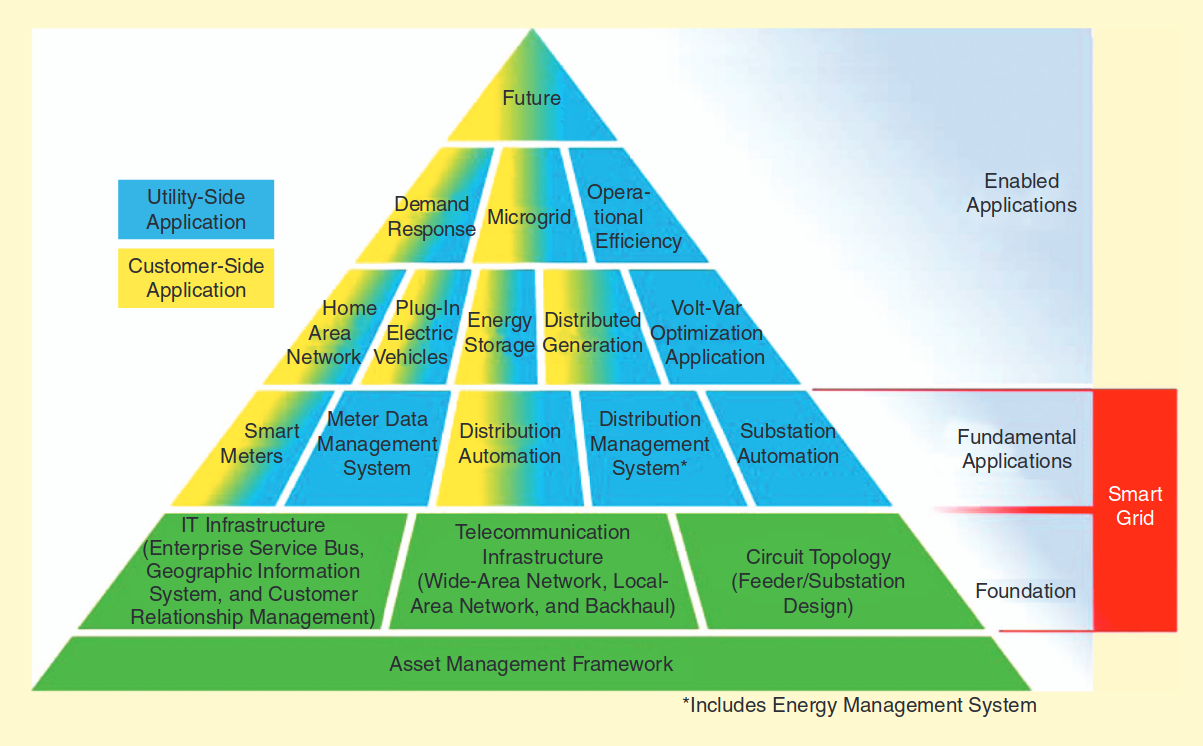
\includegraphics[width=0.74\linewidth]{PDIS/State of the Art/figures/smart_grid.png}
    \caption{Smart Grid Pyramid \cite{farhangiPathSmartGrid2010}}
    \label{fig:smart-grid}
\end{figure}


The \textit{Smart Grid} or the \textit{Smart Power Grid} conceptualizes this modernization of the electricity network by leveraging the technological advancements in information technology and communication science to create intelligent systems that manage and monitor the distributed generation of energy \cite{bayindirSmartGridTechnologies2016, farhangiPathSmartGrid2010}. Figure \ref{fig:smart-grid} describes the smart grid pyramid with asset management at its base. On this base, the foundation of the smart grid is laid out by the circuit topology, \acs{IT} systems and telecommunications infrastructure, the basic ingredients for the emergence of the fundamental applications such as smart meters and distribution automation \cite{farhangiPathSmartGrid2010}. In turn, these serve as building blocks for creating more intelligent systems that leverage upper-layer applications, enabling the true smart grid capabilities \cite{farhangiPathSmartGrid2010}.


\section{Related Works}

\ac{GRL} or Reinforcement Learning on Graphs is a relatively new area in the broader field of machine learning. \ac{GRL} techniques have shown significant progress in solving problems with underlying graph-based representations such as power grid management \cite{liNovelGraphReinforcement2022, chenGraphRepresentationLearningbased2023}, smart transport \cite{xingBilevelGraphReinforcement2023, almasanDeepReinforcementLearning2022} or task offloading \cite{gaoFastAdaptiveTask2023, liGraphReinforcementLearningbased2022}. In this work, the main focus lies on studying the development of \ac{GRL} techniques and subsequent application to smart grid services such as dynamic economic energy dispatch systems \cite{chenScalableGraphReinforcement2023, xingRealtimeOptimalScheduling2023}, residential electricity behavior identification and energy management \cite{chenGraphRepresentationLearningbased2023}, or Volt-VAR regulation \cite{huMultiagentGraphReinforcement2024}.  \par
Research on this topic has significantly increased in the last few years with the improvements of \ac{DRL} techniques and the developments in \acp{GNN} in the mid-2010s \cite{kipfSemiSupervisedClassificationGraph2017, velickovicGraphAttentionNetworks2018, liGatedGraphSequence2016, gaoGraphUNets2019}. \acp{GNN} became the state-of-the-art for solving numerous data mining tasks involving graph-structured data, excelling at classification, link prediction and representation learning \cite{xuHowPowerfulAre2019, nieReinforcementLearningGraphs2023}. This advancement brought more sophisticated \ac{RL} applications on graphs and the surge of a new field studying how to combine the improvements of graph mining and reinforcement learning techniques. \par
In this context, this literature review is divided into the two main approaches in \ac{GRL}, which compromise the popular \ac{GCN} architecture that has been widely researched or leveraging the rising and promising \ac{GAT} architecture. Lastly, other relevant approaches that use different architectures are also listed.


\subsubsection{Plain GCN-Based GRL Techniques}

A common approach in Graph Reinforcement Learning model implementation is the use of graph convolutions with the \acp{GCN} architecture for leveraging graph-based structures to extract and aggregate the essential features of data in hand and improve the performance of \ac{RL} agents in those environments. The techniques listed in this subsection constitute approaches that integrate a \ac{GCN} with \ac{RL} algorithms.\par
\cite{liNovelGraphReinforcement2022} implements a \ac{GRL} system to improve the decision quality of economic dispatch under high penetration of distributed energy generations. To accomplish this, a \ac{SAC} system is employed with the main objective of finding the optimal action policy for minimizing generation cost with the appropriate reliability concerns. This problem is represented by an undirected graph with nodes describing the power grid elements with their respective attributes and edges describing the underlying energy connections between those units. To extract the structural features of the graph, this work implements a full connected layer to perform feature transformation with a two-layer \ac{GCN} followed by three full connected layers for the non-linear mapping of state-to-action policy in both actor and critic modules. \cite{chenScalableGraphReinforcement2023} develops a similar approach, with both concluding that it significantly reduces learning time for achieving better training results in comparison to plain \ac{SAC} and showing significant improvement on economy and flexibility of the system on more complex and sparse state graphs. The use of \acp{GCN} enables the system to adapt to changes in the state space by leveraging the network's generalization ability.\par
In \cite{xingGraphReinforcementLearningBased2023} a three-layer \ac{GCN} is used to extract node feature and graph topology information and is integrated into a Rainbow-based \cite{hesselRainbowCombiningImprovements2018} \ac{DRL} algorithm for electric vehicle charging guidance. In this article, the testing results show promising performance in reducing operation costs for electric vehicle users, portraying a model with good generalization ability in untrained scenarios. \par
Another interesting implementation of this approach is \cite{chenAutonomousExplorationUncertainty2020}, which studies and compares different solutions for optimizing autonomous exploration under uncertain environments. It analyzes combinations of a single agent Deep Q-Network (DQN) and Advantageous Actor-Critic (A2C) with Graph Convolutional Networks, Gated Graph Recurrent Networks and Graph U-Nets. The paper reports that the GCN-DQN was the model that achieved the highest reward during policy training, followed by the GGNN-A2C model, although in the end, it concludes that the second showed improved scalability in relation to the first model. In \cite{chenGraphRepresentationLearningbased2023} a DQN with a GCN is also used for residential electricity behaviour identification and energy management.

\begin{table}[h!]
\centering
\caption{GCN-Based GRL Techniques}
\begin{tabular}{|P{2cm}|P{2cm}|p{5cm}|  }
 \hline
 \textbf{Reference} & \textbf{DRL Algorithm} & \textbf{Application Domain} \\
 \hline
 \cite{liNovelGraphReinforcement2022}, \cite{chenScalableGraphReinforcement2023} & GCN-SAC & Dynamic economic energy dispatch \\ \hline
 \cite{lengGraphConvolutionalNetworkbased2021} & GCN-SAC & Multi-access Edge Computing \\ \hline
\cite{yanAutomaticVirtualNetwork2020} & GCN-A3C & Automatic Virtual Network Embeddings \\ \hline
\cite{wangGCNRLCircuitDesigner2020} & GCN-DDPG & Automatic transistor sizing \\ \hline
\cite{chenAutonomousExplorationUncertainty2020} & GCN-DQN  & Autonomous Exploration under uncertainty \\  \hline
\cite{chenGraphRepresentationLearningbased2023} & GCN-DQN & Residential electricity behavior identification and energy management \\ \hline
 \cite{xingGraphReinforcementLearningBased2023} & GCN - Modified Rainbow & Electrical Vehicle Charging Guidance \\ \hline
\cite{yuanXGNNModelLevelExplanations2020} & GCN-MDP & Interpret GNNs at model-level \\ \hline
\cite{tangDependentTaskOffloading2020} & GCN-DQ & Task Offloading in Edge Computing \\ \hline
\end{tabular}
\end{table}




\subsubsection{Attention-based GRL Techniques}
Another effective approach in extracting relevant topology and graph features relies on using attention mechanisms to weigh different nodes' contributions dynamically. While this encompasses techniques that use the \ac{GAT} architecture, which is a \ac{GNN} design with the attention mechanism at its core, various scholars propose \ac{GCN} approaches integrated with attention mechanisms such as \cite{zhaoLearningSequentialDistribution2022} and \cite{fanAttentionBasedMultiAgentGraph2023}.
\cite{xingRealtimeOptimalScheduling2023} proposes a \ac{DDPG}-based algorithm improved with a \ac{GAT} block with three graph Attention Layers for extracting and learning the topology information for achieve real-time optimal scheduling for \acp{ADN}. This paper compares the obtained test results against a \ac{GCN}-\ac{DDPG} model and shows increased performance over the \ac{GCN} method in reducing cost and power loss. Beyond this, the work demonstrates that the \ac{GAT}'s attention mechanism enables the algorithm to focus on more important nodes and improve the signal-to-noise ratio compared to its \ac{GCN} counterpart. \cite{chenPhysicalassistedMultiagentGraph2023} and propose a multi-agent approach to the same domain but more focused on voltage regulation with a multi-agent \ac{SAC} instead of a single-agent \ac{DDPG} algorithm. \par
In \cite{xingBilevelGraphReinforcement2023}, another model for the electric vehicle charging guidance is proposed, consisting of a bi-level approach of a Rainbow-based algorithm with a \ac{GAT} block. The upper level focuses on the decision-making process regarding charging, while the lower level handles routing. The proposed model proved to be more effective than a shortest distance path-based \cite{xingModellingDrivingCharging2021} and a \ac{DRL}-based \cite{qianDeepReinforcementLearning2020} approach. It suggests that in a future direction, developing \acp{GNN} directly embedded into the \ac{RL} framework might further improve the model's robustness and scalability. \cite{xuRealtimeFastCharging2022} develops a similar approach with a Double-prioritized DQN for the same application domain.
In \cite{zhaoLearningSequentialDistribution2022} and \cite{fanAttentionBasedMultiAgentGraph2023}, the sequential distribution system restoration problem is addressed with a multi-agent \ac{RL} algorithm equipped with a \ac{GCN} with an attention mechanism. In the first case, multi-head attention is used as the convolution kernel for the \ac{GCN} with a \ac{DQN} algorithm. In the second, self-attention is used for improving the centralized training of the used multi-agent actor-critic algorithm, more concretely, by embedding it in the critic networks. At the same time, the \ac{GCN} is integrated into the actor networks for extracting the graph features. Both solutions proved more efficient than traditional \ac{RL} techniques, with the first highlighting its solution generalizability and the second showing increased scalability facing the non-GRL techniques.


\begin{table}[h!]
\centering
\caption{Attention-Based GRL Techniques}
\begin{tabular}{|P{2cm}|P{4cm}|p{6cm}|  }
 \hline
 \textbf{Reference} & \textbf{DRL Algorithm} & \textbf{Application Domain} \\
 \hline
 \cite{xingRealtimeOptimalScheduling2023} & GAT-DDPG & Optimal Scheduling for ADNs  \\ \hline
  \cite{chenPhysicalassistedMultiagentGraph2023}  &  GAT-MASAC  & Multi-agent Voltage Regulation \\ \hline 
 \cite{xingBilevelGraphReinforcement2023} & GAT-Modified Rainbow & Electric Vehicle Charging Guidance \\ \hline
 \cite{xuRealtimeFastCharging2022} & GAT-DQN & Electric Vehicle Charging Guidance \\ \hline 
 \cite{zhaoLearningSequentialDistribution2022} & GCN-DQN & Multi-agent Sequential Distribution System Restoration \\ \hline
 \cite{fanAttentionBasedMultiAgentGraph2023} & GCN-MAAC & Multi-agent Service Restoration \\ \hline
\end{tabular}
\end{table}


\subsubsection{Other Approaches}

This subsection includes \ac{GRL} approaches that combine of other \acp{GNN} architectures with \ac{RL} algorithms. In \cite{peiEmergencyControlStrategy2023}, a GraphSAGE network is used with a Deep Dueling Double Q-Network (D3QN) for emergency control of Undervoltage load shedding for power systems with various topologies. The author presents promising results for the GraphSAGE-D3QN model compared to a GCN-D3QN, achieving higher cumulative reward and faster voltage recovery speed, although it required longer decision times. The proposed model performed excellently in the application domain and successfully generalised the learned knowledge to new topology variation scenarios. \par
\cite{zhangLearningDispatchJob2020} focused on solving the Job shop scheduling problem through a priority dispatching rule with a Graph Isomorphism Network \cite{xuHowPowerfulAre2019} and an actor-critic \ac{PPO} algorithm where the GIN is shared between actor and critic networks. The method showed superior performance against other traditional manually designed priority dispatching rule baselines, outperforming them by a large margin.

\begin{comment}
GCN

\cite{yanGraphCooperationDeep2023} & GCN-DQN & GRU, Multi-agent and Multi-head Attention & Ecological Traffic Signal Control \\ \hline

\cite{luoMultiAgentCollaborativeExploration2019} & GCN-DQN & & Autonomous Exploration under uncertainty \\ \hline

Attention
\cite{huMultiagentGraphReinforcement2024} & HRGN-MASAC & Multi-agent Vol-VAR Regulation \\ \hline

\end{comment}

\subsection{Conclusion}

In conclusion, \ac{GRL} is very promising field, where several different applications and techniques were already studied. \acp{GNN} architectures such as \ac{GCN} have been extensively applied with DRL algorithms for enabling feature extracting from graph-based state representations \cite{chenScalableGraphReinforcement2023, chenAutonomousExplorationUncertainty2020}. Architectures such as the GraphSAGE and other attention-based have also been successfully applied with very promising results \cite{peiEmergencyControlStrategy2023, xingRealtimeOptimalScheduling2023} in comparison with \acp{GCN}. However, less research regarding their integration with DRL algorithms was discovered. This suggests that a possible improvement and research direction in the development of \ac{GRL} techniques might be connected with exploring the use of different \acp{GNN} architectures and using the rising attention-based techniques.



%% the references using BibTeX
\bibliographystyle{unsrt}
\bibliography{sota}

\end{document}
